\chapter{Grundlagen}
\label{chap:grundlagen}
Container werden häufig als leichtgewichtige \glspl{acr-vm} beschrieben. Dies ist allerdings nicht ganz richtig. Wie in \fref{fig:containerVsVm} zu erkennen, virtualisieren Container kein vollständiges \gls{acr-os}, sondern lediglich das benötigte Dateisystem. Dabei wird der Kernel des Hosts nicht virtualisiert, sondern mitverwendet. Dies macht Container deutlich leichtgewichtiger als \glspl{acr-vm}, isoliert allerdings weniger umfangreich als diese. So werden bei Containern Kernelfunktionen mit dem Host-\gls{acr-os} geteilt. \glspl{acr-vm} isolieren diese Funktionen in eigenen virtuellen Betriebssystemen.
\begin{figure}[h]
		\subfigure[Container]{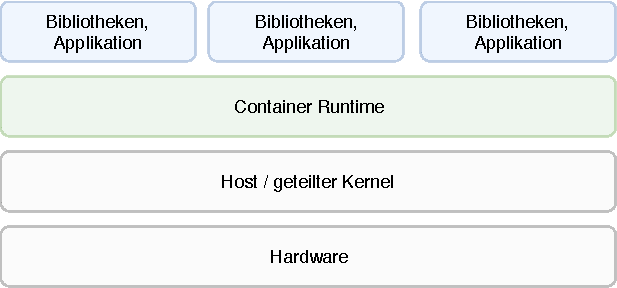
\includegraphics[width=0.49\textwidth]{bilder/container-stack-isolation.pdf}}
		\hfill
		\subfigure[\glspl{acr-vm}]{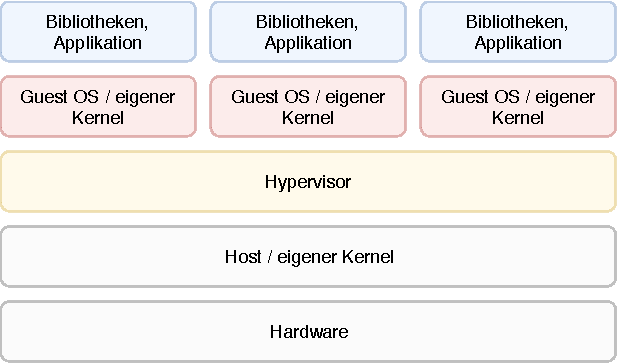
\includegraphics[width=0.49\textwidth]{bilder/vm-stack-virtualisation.pdf}}
		\caption{Container Isolation im Vergleich zu \glspl{acr-vm}}
		\label{fig:containerVsVm}
\end{figure}

Dieses Kapitel behandelt alle benötigten Grundlagen, die zur Isolation eines Prozesses benötigt werden. Es werden vorhandene Standards wie die \gls{acr-oci} und benötigte Systemcalls wie \gls{acr-chroot} näher erläutert. Zudem wird beschrieben, wie die Isolation, die Container bieten, durch Systemmittel des Linux-Kernels selber erreicht werden kann.
\section{Standards}
\label{sec:standards}
Durch die immer größere Verwendung von Containern und die Verbreitung verschiedener Container-Runtimes ist die Standardisierung eine wichtige Aufgabe. Folgend werden Standardisierungsprojekte aufgezählt, die bestehenden Spezifikationen erläutert und aktuelle Aufgaben der Projekte näher betrachtet.
\subsection{App Container}
\label{sec:appc}
\Gls{acr-appc} ist ein Standard, der viele Aspekte innerhalb der Container-Landschaft behandelt. Dabei liegt die Hauptaufgabe darin, eine Laufzeitumgebung wie auch das \gls{gls-image}-Format und die Verbreitung von \glspl{gls-image} zu spezifizieren. Seit 2016 wird das Projekt nicht mehr aktiv weiterentwickelt, da mit der Gründung der \gls{acr-oci} ein größeres Standardisierungsprojekt entstand. Bestandteile der \gls{acr-appc} wurden von der \gls{acr-oci} übernommen und dienen als Vorlage für die Spezifikation dieser.

\subsection{Open Container Initiative}
\label{sec:oci}
Die \gls{acr-oci} ist eine Initiative, die seit 2015 unter der Linux Foundation agiert. Das Ziel der OCI ist es, einen offenen Standard für Container zu schaffen, sodass die Wahl der Container-Laufzeitumgebung nicht mehr zu Inkompatibilität führt. Dabei liegt der Fokus auf eine einfache, schlanke Implementierung \citep{OpenContainerInitiative}. 

Die OCI arbeitet aktuell an zwei Spezifikationen. Die runtime-spec standardisiert die Laufzeitumgebung  von Containern. Dabei wird festgelegt, welche Konfiguration, Prinzipien und Schnittstellen Laufzeitumgebungen stellen müssen. Um die Umsetzung der runtime-spec zu fördern, stellt die OCI eine beispielhafte Implementierung durch runC. Das zweite Projekt der OCI ist die image-spec. Dieses versucht einen Standard für \glspl{gls-image} zu definieren. Dabei plant die OCI nicht, vorhandene Image-Formate zu ersetzen, sondern auf diesen Aufzubauen und sie zu erweitern \citep{OpenContainerInitiative}.
\begin{table}[h]
	\begin{center}
		\begin{tabular}{lcccc}
			\toprule
			& \multicolumn{2}{c}{Standard} & \multicolumn{2}{c}{Container Runtime}\\
			\cmidrule{2-5}
			& OCI		& appc		& Docker			& rkt					\\
			\midrule
			Container Image			& \faTimes	& \faCheck	& OCI image-spec 	& appc Image Format		\\
			Image Verbreitung		& \faTimes	& \faCheck	& Docker Registry	& appc Discovery Spec 	\\
			Lokales Speicherformat	& \faCheck	& \faTimes	& keine Spezifikation& keine Spezifikation	\\
			\midrule
			Runtime					& \faCheck	& \faCheck	& runC 				& appc runtime Spec		\\
			\bottomrule
		\end{tabular}
	\end{center}
	\caption{Standards OCI und AppC im Vergleich \citep{MakingSenseofContainerStandardsandFoundations:OCICNCFAppcandRkt}}
	\label{tab:ociVSappc}
\end{table}

Wie in \fref{tab:ociVSappc} zu sehen, wurden einige Konzepte des \gls{acr-appc}-Projekts in die \gls{acr-oci} übernommen. Vor allem die \gls{gls-image}-Spezifikation wurde durch die Mitarbeit ehemaliger \gls{acr-appc}-Maintainer gefördert. Allerdings sind einige Projekte noch nicht übernommen worden. So gibt es keine \gls{acr-oci} Spezifikation für die Verbreitung von \glspl{gls-image}, eines der meistgenutzten Features verschiedener Container-Runtimes. Um die Weiterentwicklung an solchen Projekten zu fördern wurden einige in die \gls{acr-cncf} übernommen \citep{MakingSenseofContainerStandardsandFoundations:OCICNCFAppcandRkt}.

\subsection{Cloud Native Computing Foundation}
\label{sec:cncf}
Die \gls{acr-cncf} beschäftigt sich im Gegensatz zur \gls{acr-oci} nicht nur mit Containern, sondern der kompletten \gls{gls-cn}-Landschaft. Projekte wie \gls{acr-k8} und Prometheus werden durch die \gls{acr-cncf} weiterentwickelt und publiziert \cite{}. Da der Cloud-Native Entwicklungsprozess von Containern getragen wird, spielen Technologien wie containerd und rkt eine entscheidende Rolle für die \gls{acr-cncf}. Neben Container-Runtimes beinhaltet die \gls{acr-cncf} auch Projekte zur Orchestrierung von Containern, Logging und Monitoring dieser, wie auch Spezifikationen, zum Beispiel die TUF, eine Spezifikation die standardisiert, wie Softwarepakete upgedatet werden sollen \cite{CNCFCloudNativeInteractiveLandscape}.

\begin{figure}[h]
	\begin{center}
		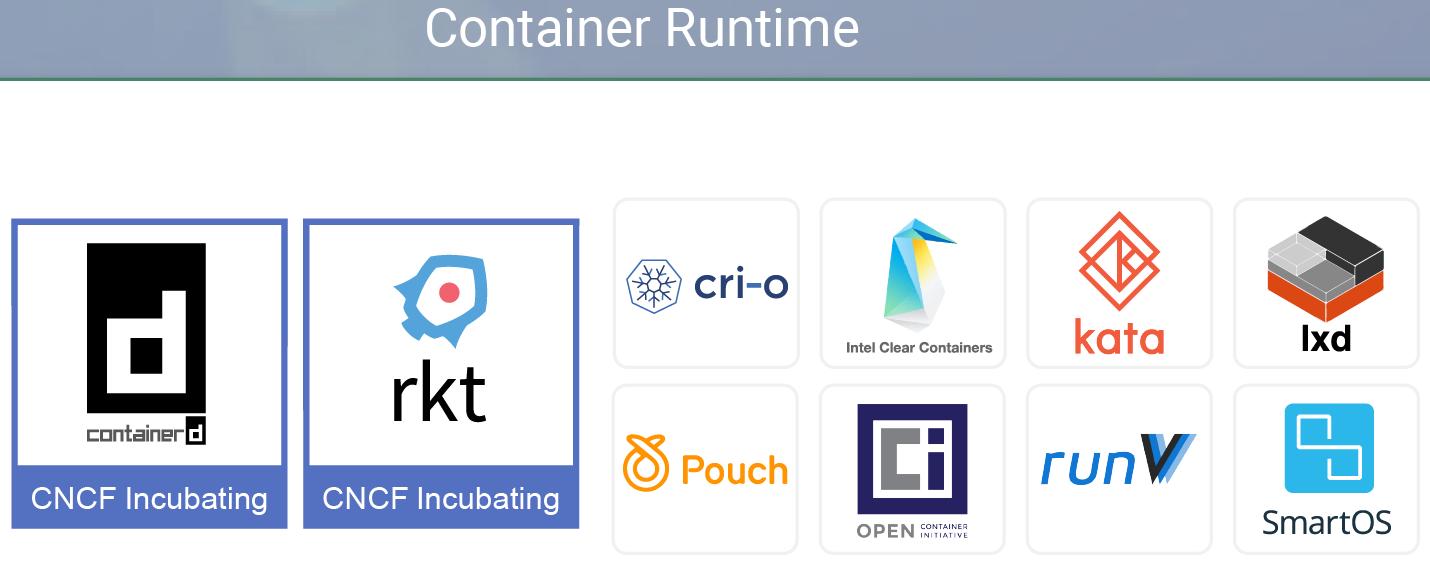
\includegraphics[scale=0.3]{bilder/cncf-container-landscape.png}
		\caption{CNCF Container Runtime Landschaft \citep{CNCFCloudNativeInteractiveLandscape}}
		\label{fig:cncfContainerLandscape}
	\end{center}
\end{figure} 

\section{Funktionsweise}
\label{sec:funktionsweise}

Container isolieren einzelne Prozesse durch verschiedene Kernel-Technologien, die im Folgenden erklärt werden sollen.
\subsection{Change Root}
\label{sec:chroot}
\Gls{acr-chroot} ist ein Unix Systemaufruf, der es erlaubt einen Prozess in einem anderen Wurzelverzeichnis auszuführen \citep{Chroot1LinuxManualPage}. Daraus folgt, dass der Prozess in einer eigenen Verzeichnisstruktur arbeitet und keine Dateien des Host-\gls{acr-os} ändern kann. \Gls{acr-chroot} erlaubt somit die Isolierung des Dateisystems, die Container nutzen.

\subsection{Control Groups}
\label{sec:cgroups}
\Glspl{acr-cgroup} dienen dazu, Systemressourcen für einzelne Prozesse zu limitieren. \Glspl{acr-cgroup} sind anders als \gls{acr-chroot} kein Unix-Feature sondern Teil des Linux-Kernels. Im \gls{acr-os} sind \glspl{acr-cgroup} als Dateihierarchie repräsentiert. Das gesamte \gls{acr-cgroup}-Dateisystem ist unter \texttt{/sys/fs/cgroup/} zu finden.

\Glspl{acr-cgroup} stellen zur Steuerung verschiedene Controller zur Verfügung.
\begin{table}[H]
	\begin{center}
		\begin{tabular}{ll}
			\toprule
			Controller 	& Ressource 												\\
			\midrule
			io			& Zugriff und Nutzung von Block Geräten wie Festplatten		\\
			memory		& Monitoring und Beschränken des Arbeitsspeichers 			\\
			pids		& Limitierung der Anzahl an Unterprozessen					\\
			perf\_event	& Erlaubt Performance Monitoring der Prozesse				\\
			rdma		& Zugriffe über RDMA limitieren oder sperren				\\
			cpu			& CPU-Zyklen und maximale CPU-Bandwidth						\\
			\bottomrule
		\end{tabular}
		\caption{\Glspl{acr-cgroup}-Controller und deren Verwendung \citep{Cgroups7LinuxManualPage}}
		\label{tab:cgroupController}
	\end{center}
\end{table}

\subsection{Namespaces}
\label{sec:namespaces}
Namespaces abstrahieren einzelne Bereiche des \gls{acr-os}. Sie werden genutzt, um globale Ressourcen zu isolieren. Ein Namespace kapselt dabei einzelne Ressourcen. Veränderungen an diesen sind für alle Prozesse innerhalb desselben Namespaces sichtbar, allerdings außerhalb dieses unsichtbar \citep{Namespaces7LinuxManualPage}.

\begin{table}[h]
	\begin{center}
		\begin{tabular}{ll}
			\toprule
			Namespace			& Ressource				 				\\
			\midrule
			\Gls{acr-cgroup}	& \Gls{acr-cgroup}-Dateisystem 			\\
			IPC					& System V IPC, POSIX Nachrichten 		\\
			Network				& Netzwerk Geräte, Stacks, Ports, ...	\\
			Mount				& Mount Punkte							\\
			PID					& Prozess IDs							\\
			User				& Nutzer und Gruppen IDs				\\
			UTS					& Hostnamen und Domänennamen			\\
			\bottomrule
		\end{tabular}
	\end{center}
	\caption{Linux Namespaces und verbundene Ressourcen \citep{Namespaces7LinuxManualPage}}
	\label{tab:namespaces}
\end{table}

\subsection{Mounting}
\label{sec:mount}
Durch die Isolation eines Prozesses und die Bedingung, das Container unveränderlich sein sollen stellt sich die Frage, wie man Containern Dateien aus dem Host-System zur Verfügung stellt. Dies ist vor allem wichtig, wenn bei Veränderung der Umgebung nicht den Container neu gestartet werden soll. Sollte zum Beispiel eine neue Datei durch einen Webserver zur Verfügung gestellt werden, möchte man nicht den Container neu starten. Die Lösung dieses Problems ist der Unix-Systembefehl \texttt{mount}. 

Mit diesem Befehl wird eine beliebige Dateihierarchie an eine andere Stelle des Dateibaums angeheftet. Durch dieses vorgehen kann man Ordner vom Host-System  für das mit \gls{acr-chroot} isolierte Dateisystem des Containers zugänglich machen. Dabei ist zu beachten, dass es sich bei dem gemounteten Ordner nicht um einen symbolischen Link handelt. Diese könnten durch den Aufruf von \texttt{chroot} nicht mehr aufgelöst werden.

\begin{figure}[h]
	\centering
	\begin{minipage}{0.9\textwidth}
		\dirtree{%
			.1 /home.
			.2 rootfs.
			.3 var.
			.4 src.\DTcomment{mounted von \texttt{/home/readonly/} }.
			.5 \color{red}hungry.py.\DTcomment{kein symbolischer Link}.
			.5 \color{red}port.py.\DTcomment{kein symbolischer Link}.
			.3 \vdots.
			.2 readonly.
			.3 \color{red}hungry.py.
			.3 \color{red}port.py.
		}
	\end{minipage}
	\caption{Auszug aus Dateisystem mit gemounteten Dateien}
	\label{fig:mountExample}
\end{figure}

\subsection{Netzwerk}
\label{sec:netzwerk}

Einen weiteren Aspekt, den Container vom Host-\gls{acr-os} isolieren ist das Netzwerk. Dabei kommen virtuelle Ethernet-Adapter zum Einsatz. Diese erlauben es, ein unabhängiges Netzwerk zu erzeugen. Ein Ende des \gls{acr-veth} wird dabei der PID des Containers zugewiesen, das andere dem Host. Zusätzlich wird der Network-Namespace genutzt um eine vollständige Isolation des Netzwerks zu erhalten.

\begin{figure}[h]
	\begin{center}
		\missingfigure{Netzwerk Graph für Container und Host?}
		\caption{Netzwerkseparation zwischen Host und Container}
		\label{fig:networkContainer}
	\end{center}
\end{figure}

\subsection{Sicherheit}
\label{sec:sicherheit}

\begin{quote}
	\textit{"Docker is about running random code downloaded from the Internet and running it as root"}
	\flushright
	\small{---Dan Walsh (Red Hat)}
\end{quote}

Container haben ein großes Problem. Alle genannten Kernel-Features müssen als Nutzer \texttt{root} ausgeführt werden. Dadurch haben die gestarteten Prozesse häufig Berechtigungen, die es erlauben würden, aus der Isolierung des Containers auszubrechen. Um dies zu verhindern, können verschiedene Sicherheitskonzepte verwendet werden.

Das leichteste dieser Konzepte sind Capabilities. Jeder Prozess, sowie jeder Datei kann eine Liste an Capabilities zugeordnet oder genommen werden. Dabei können einzelnen Dateien beispielsweise die Rechte genommen werden, auf Port 80 zu hören. Auch viele Systemaufrufe können über Capabilites gewährt oder verwehrt werden. Ein anderes Konzept ist die Implementation eines \textit{Mandatory Access Control}-Systems wie SELinux oder AppArmor. Diese Implementationen sind granularer als Capabilites, allerdings mit einem höheren Konfigurationsaufwand verbunden.

\subsection{Container unter Windows}
\label{sec:windows}
Bislang wurden Container nur unter Linux verwendet. Viele Kernel-Features des Linux-Kernels erlauben eine Isolation und wurden teilweise spezifisch für diese entwickelt \citep{Namespaces7LinuxManualPage}. Seit 2016 können spezifisch Docker-Container auch unter Windows genutzt werden. Dabei trennt Microsoft Container in zwei verschiedene Isolationen auf.

Hyper-V Container, die unter Windows 10 genutzt werden sind extrem abgespeckte Hyper-V \glspl{acr-vm}, die nur noch nötigste Features einer \gls{acr-vm} behalten. Dabei wird, nicht wie in \fref{fig:containerVsVm} dargestellt auch der Kernel virtualisiert. Die zweite Alternative basiert auf Windows Server 2016 Container, die nur unter Windows Server 2016 und neueren Windows Server Betriebssystemen funktionieren. Diese implementieren eine wirkliche Isolation durch den Windows-Kernel.

\section{Eigene Implementierung}
\label{sec:eigeneImpl}
Um die in \fref{sec:funktionsweise} erläuterten Kernel-Features näher zu beleuchten wird folgend gezeigt, wie ein Prozess isoliert vom Host-System ausführen kann. Dabei wird darauf eingegangen, wie ein Tarball durch das Tool buildroot erstellt werden kann, was am Beispiel der Python-Runtime gezeigt wird. Dieser lässt sich folgend in Container-Runtimes wie \gls{acr-rkt} importieren. Im Folgenden wird dieser mithilfe der Kernel-Funktionen aus \fref{sec:funktionsweise} isoliert. Das Ergebnis ist ein Dateisystem innerhalb eines Host-\gls{acr-os}, indem  eine Instanz der Python-Runtime isoliert und ohne Root-Berechtigungen ausgeführt wird.

\subsection{Erstellen eines tarballs}
\label{sec:tarball}
Bei einem tarball handelt es sich um ein komprimiertes Dateisystem. Dabei wird ein vollwertiges Linux-Dateisystem stark komprimiert, um es leichter zu versenden oder zusichern. Das Erzeugen eines tarballs ist durch das Tool buildroot einfach. Buildroot ist ein Unix-Tool, welches zur Erstellung von minimalistischen Linux-Distributionen für Embedded-Systems entworfen wurde. Es erlaubt aber auch, nur ein Dateisystem zu erzeugen, ohne Kernel oder Init-System. Dies ist entscheidend, da bei Containern der bestehende Kernel des Host-OS mitbenutzt wird (\textit{siehe \fref{fig:containerVsVm}}. Das Init-System, welches dazu dient, neue Prozesse zu starten, wird in einem Container ebenfalls nicht benötigt, da diese nur einen Prozess ausführen. Diese Features von buildroot erlaubt es, ein \gls{gls-image} für Container zu erzeugen.

\begin{figure}[h]
	\begin{center}
		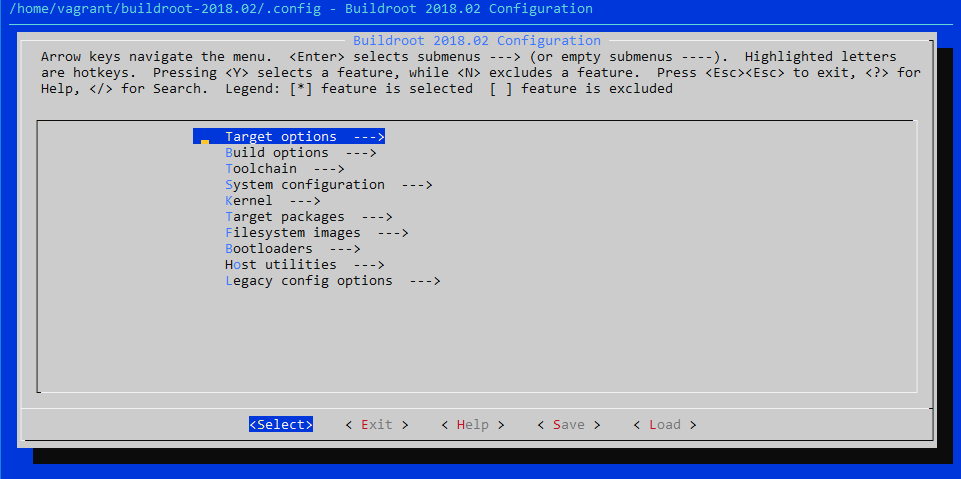
\includegraphics[scale=0.5]{bilder/buildroot-menuconfig.png}
		\caption{Buildroot Menü nach Start des Tools}
		\label{fig:buildrootMenuConfig}
	\end{center}
\end{figure}

Zudem erlaubt es buildroot, einzelne Bibliotheken, wie zum Beispiel die Python-Runtime, beim Build-Prozess der Distribution zu integrieren. Nach dem Einstellen der benötigten Bibliotheken und dem deaktivieren der, für Container, unnötigen Features erzeugt Buildroot eine Config-Datei, die all3 Änderungen beinhaltet. Durch das Starten des Build-Prozesses mit dem Befehl \texttt{make} wird die gewünschte Linux-Distribution erstellt.

Am Ende dieses Prozesses liegt im Ordner \texttt{/buildroot/out/images/} das gewünschte Dateisystem \texttt{rootfs.tar}.

\subsection{Isolieren der Python-Runtime}
\label{sec:isolieren}
In \fref{sec:tarball} wurde ein Dateisystem mit der Python-Runtime erstellt. Dieses muss nun isoliert, ein Pythonprogramm in das Dateisystem gemounted und ausgeführt werden.

Der erstellte tarball wird durch folgende \gls{gls-bash}-Befehle entpackt. 

\begin{listing}[h]
	\begin{minted}[xleftmargin=-75pt]{bash}
		cd /home
		mkdir rootfs
		cp rootfs.tar rootfs/
		cd rootfs
		sudo tar xvf rootfs.tar
		sudo rm rootfs.tar
	\end{minted}
	\caption{Entpacken des buildroot tarballs nach /home/rootfs}
	\label{lst:untarRootfs}
\end{listing}


\begin{figure}[h]
	\centering
	\begin{minipage}{0.9\textwidth}
		\dirtree{%
			.1 /home/rootfs/.
			.2 usr.
			.3 bin.
			.4 python -> python3.6.\DTcomment{nicht aus Hostsystem}.
			.4 python3.6.
			.3 \vdots.
			.2 \vdots.
		}
	\end{minipage}
	\caption{Dateibaum nach entpacken der \texttt{rootfs.tar}}
	\label{fig:baumNachUntar}
\end{figure}

Um einen Prozess mit dem Wurzelverzeichnis \texttt{/home/rootfs/} auszuführen, ist lediglich der folgende Aufruf nötig.
\begin{listing}[h]
	\begin{minted}[xleftmargin=-75pt, breaklines, breakafter=/]{bash}
		sudo chroot rootfs /usr/bin/python3.6 -m http.server
	\end{minted}
	\caption{Shell-Commands um Python Webserver mit definierter Wurzel zu starten}
	\label{lst:pythonChrooted}
\end{listing}

Durch diesen wird ein Webserver auf Adresse \texttt{http://0.0.0.0:8000} ausgeführt, der alle ihm zugänglichen Dateien zum Download bereitstellt. Beim Aufrufen dieser Adresse erkennt man, dass der Webserver nur Zugriff auf die in \texttt{/home/rootfs/} liegenden Dateien hat.

\begin{figure}[H]
	\begin{center}
		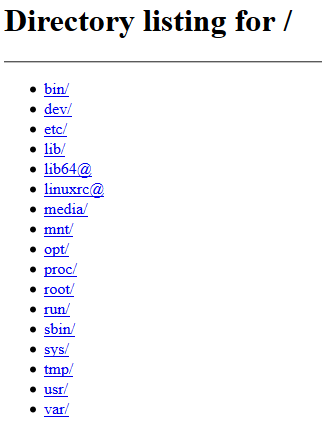
\includegraphics[scale=0.8]{bilder/chroot-python-webserver.png}
		\caption{Python Webserver mit festgesetztem Root-Verzeichnis}
		\label{fig:chrootPythonWebserver}
	\end{center}
\end{figure}

Um weiterhin Zugriff auf dynamische Inhalte aus dem Host-System zu haben, kann man, wie in \fref{sec:mount} entsprechende Verzeichnisse in das neue \texttt{rootfs} des Prozesses mounten.

\begin{listing}[h]
	\begin{minted}[xleftmargin=-75pt]{bash}
		nsenter --mount=/proc/<PID isolierter Prozess>/ns/mnt \
			mount --bind -o ro \
				$PWD/readonly \
				$PWD/rootfs/var/src
	\end{minted}
	\caption{Mounten von Verzeichnis \texttt{/readonly/} zu \texttt{/rootfs/var/src/}}
\end{listing}

Durch die Dateitrennung und den aufruf von \texttt{chroot} tritt allerdings ein großes Problem aus. Der Python-Webserver wird mit erhöhten Rechten ausgeführt, da diese für den Aufruf von \texttt{chroot} benötigt werden.

\begin{figure}[h]
	\begin{center}
		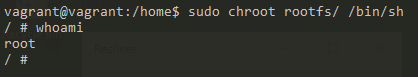
\includegraphics[scale=1]{bilder/chroot-whoami-root.png}
		\caption{Root-Eskalation durch Aufruf von \texttt{sudo chroot}}
		\label{fig:chrootWhoami}
	\end{center}
\end{figure}

Dies führt zu vielen Problemen. Ein Prozess, der nur auf diese Weise isoliert wird, könnte beispielsweise Prozesse auf dem Hostsystem mit \texttt{kill <pid>} beenden. Die Lösung dieses Problems sind die in \fref{sec:namespaces} beschriebenen namespaces.

Um alle Prozesse des Hostsystems vor dem Container zu verstecken, muss der PID-Namespace des Container-Prozesses neu gemounted werden.
\begin{listing}[h]
	\mintinline{bash}{sudo unshare -p --mount-proc=\$PWD/rootfs/proc -f chroot rootfs /bin/sh}
	\caption{Remount des PID-Namespaces und Chroot einer Shell}
\end{listing}

Beim Aufruf von "\mintinline{bash}{ps aux}" wird nur noch der Prozess \texttt{/bin/sh} angezeigt, der die PID 1 bekommen hat. Dieses Vorgehen löst allerdings nicht die Wurzel des Problems. Der gestartete Prozess läuft auch weiterhin unter dem Nutzer root. Ein auf diese Weise isolierter Prozess, kann zum Beispiel auf Port 80 hören. Um diese Berechtigungen zu entfernen werden die in \fref{sec:sicherheit} angesprochenen Capabilites verwendet.

\begin{listing}
	\begin{minted}[xleftmargin=-75pt,breaklines, breakafter=/]{bash}
		capsh --drop=cap_net_bind_service --chroot=rootfs/ --
	\end{minted}
	\caption{Entfernen der Capability um auf Port 80 zu hören}
\end{listing}

Durch diesen Aufruf hat, die in \texttt{rootfs} gestartete \texttt{/bin/bash} nicht mehr die Möglichkeit, auf niedrigere Ports, wie Port 80 zu hören.

Um vollständige Isolation des Containers zu erreichen, müssen allerdings auch Systemressourcen, wie Arbeitsspeicher oder CPU-Zyklen limitiert werden. Dazu dienen die in \fref{sec:cgroups} beschriebenen \glspl{acr-cgroup}.

Um eine \gls{acr-cgroup} zu erstellen, muss ein Ordner unterhalb des Wurzelverzeichnisses erstellt werden. Um einen Prozess einer \gls{acr-cgroup} zuzuordnen, wird die PID des Prozesses in die Datei \texttt{/sys/fs/cgroup/<controller>/<cgroupname>/tasks} geschrieben.

\begin{listing}[h]
	\begin{minted}[xleftmargin=-75pt, breaklines, breakafter=/]{bash}
		mkdir /sys/fs/cgroup/memory/container
		echo "1111" > /sys/fs/cgroup/memory/container/tasks
	\end{minted}
	\caption{Erzeugen einer memory cgroup namens container}
\end{listing}

Um festzusetzen, wie viel Arbeitsspeicher der isolierte Prozess nutzen darf, kann man innerhalb der \gls{acr-cgroup} einzelne Limits festlegen.

\begin{listing}[h]
	\begin{minted}[xleftmargin=-75pt, breaklines, breakafter=/]{bash}
		echo "0" > /sys/fs/cgroup/memory/container/memory.swappiness
		echo "100000000" > /sys/fs/cgroup/memory/container/memory.limit_in_bytes
	\end{minted}
	\caption{Limitieren maximaler Arbeitsspeicher und Memory-Swap deaktivieren}
\end{listing}

Um zu testen, ob die Zuweisung funktioniert und durch den isolierten Prozess maximal 100Mb Arbeitsspeicher belegt werden können, kann folgendes Python Programm ausgeführt werden. \fref{fig:cgroupKilled} zeigt die Ausgabe des Prozesses.

\begin{listing}[p]
	\begin{minted}[xleftmargin=-75pt]{python}
		#hungry.py - Eating up memory in 10Mb blocks
		import time
		
		TEN_MEGABYTE = 10000000
		
		f = open("/dev/urandom", "rb")
		data = bytearray()
		i = 0
		
		while True:
			data.extend(f.read(TEN_MEGABYTE))
			i += 1
			print("%dMb belegt" % (i*10,))
			time.sleep(1)
	\end{minted}
	\caption{Python Programm hungry.py um Arbeitsspeicher zu verbrauchen}
	\label{lst:hungry-py}
\end{listing}


\begin{figure}[p]
	 \begin{center}
	 	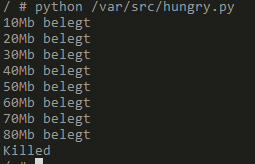
\includegraphics[scale=1]{bilder/cgroup-container-killed.png}
	 	\caption{Ausgabe des Pythonprogramms \texttt{hungry.py}}
	 	\label{fig:cgroupKilled}
	 \end{center}
\end{figure}